%!TEX root = ../../../tugas-akhir.tex
\section{\textit{Transport Layer Security} (TLS)}
  \textit{Transport Layer Security} (TLS) adalah sebuah protokol kriptografi yang menjamin kerahasiaan serta integritas dalam data yang dikirim dalam sebuah koneksi yang tidak dipercaya. TLS pertama kali dikembangkan sebagai \textit{Secure Socket Layer} (SSL) oleh Netscape pada tahun 1995, dan kemudian diresmikan oleh Internet Engineering Task Force (IETF) dalam RFC 2246 pada tahun 1998. SSL dirancang dengan empat tujuan utama yaitu keamanan secara kriptografis, interoperabilitas, kemampuan penambahan protokol, serta efisiensi \citep{perf_tls}.

  TLS dirancang sebagai sebuah protokol perantara antara protokol aplikasi (HTTP, FTP, SMTP) dan protokol transport (TCP, UDP). Semua data yang dikirimkan oleh aplikasi akan dienkripsi terlebih dahulu oleh TLS sehingga data dapat dikirimkan secara terenkripsi. Hal ini dapat mempermudah penggunaan TLS diatas protokol aplikasi mengingat aplikasi hanya perlu mengirimkan data melalui TLS socket alih-alih melalui TCP/UDP socket untuk kemudian dienkripsi dan dikirimkan pada tujuan melalui TCP/UDP socket. Ilustrasi perbandingan antara pengiriman dengan menggunakan TLS dan tidak menggunakan TLS dapat dilihat pada Gambar ~\ref{fig:tls-usage}

  \begin{figure}[h]
    \centering
    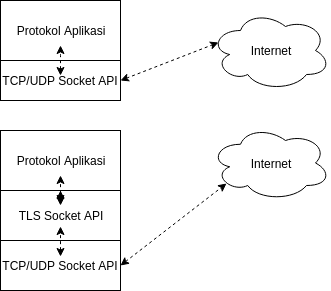
\includegraphics[width=0.6\textwidth]{resources/img/ch-2/tls-usage.png}
    \caption{Perbandingan Penggunaan Protokol TLS pada Aplikasi \protect\citep{perf_tls}}
    \label{fig:tls-usage}
  \end{figure}

  Dewasa ini, TLS umum digunakan sebagai layer keamanan pada protokol aplikasi yang umum digunakan di internet. Berbagai protokol yang awalnya tidak memiliki standar keamanan dapat menggunakan TLS untuk mengamankan aliran data. Sebagai contoh, penggunaan HTTPS dapat memastikan bahwa data-data penting seperti \textit{password}, nomor kartu kredit, ataupun alamat tidak dapat dilihat oleh siapapun kecuali pengguna dan pemilik dari sebuah website.

  TLS merupakan sebuah protokol asimetrik dimana pihak yang melakukan koneksi dapat dibagi menjadi client dan server. TLS menyediakan metode otentikasi sehingga sebuah pihak dapat yakin bahwa ia memang berkomunikasi dengan pihak yang ia inginkan. TLS menyediakan metode otentikasi baik untuk client maupun server, walaupun pada praktiknya biasanya hanya server yang diotentikasi oleh client. Salah satu metode lain adalah TLS memastikan bahwa pesan yang dikirim tidak diubah pada perjalanan dengan adanya penambahan \textit{Message Authentication Code} (MAC) pada semua data yang dikirim.

  Protokol TLS pada dasarnya tersusun dari dua protokol utama, yaitu Protokol TLS \textit{Record} dan Protokol TLS \textit{Handshake}. Protokol TLS Record digunakan untuk mengenkapsulasi data yang diterima oleh protokol aplikasi, sementara itu Protokol TLS Handshake digunakan untuk mengotentikasi client dan server serta melakukan negosiasi mengenai pemilihan penggunaan algoritma enkripsi, kunci yang digunakan, serta pemilihan penggunaan algoritma MAC (Message Authentication Code).

  % Pengembang dari TLS sadar bahwa komputasi kriptografis yang digunakan dalam otentikasi server memerlukan biaya komputasi yang cukup tinggi. Karena itulah, TLS memiliki sebuah mekanisme session yang memungkinkan client yang telah menyelesaikan TLS \textit{Handshake} sebelumnya untuk melakukan TLS Handshake secara cepat dengan menggunakan ulang data session yang masih tersimpan pada client. Pada sebuah session, data yang tersimpan diantaranya:
  % \begin{description}
  %   \item[-] \textit{Session identifier}
  %   \item[-] \textit{Peer cerficate}
  %   \item[-] \textit{Compression method}
  %   \item[-] \textit{Cipher spec}, yaitu pasangan algoritma yang digunakan dalam enkripsi dan MAC.
  %   \item[-] \textit{Master secret}, yaitu key 48-byte yang digunakan dalam enkripsi dan dekripsi.
  %   \item[-] \textit{is resumable}, menandakan apakah session ini dapat digunakan untuk membuat session baru.
  % \end{description}


  \subsection{Protokol TLS \textit{Handshake}}
    TLS \textit{Handshake} adalah protokol yang digunakan untuk melakukan otentikasi serta negosiasi untuk menentukan parameter yang digunakan pada sebuah koneksi TLS. Sebuah TLS \textit{handshake} juga digunakan untuk membuat dan menentukan \textit{session} dari sebuah koneksi TLS. Protokol ini juga mendeskripsikan cara yang digunakan oleh TLS untuk memberikan tanda pada satu sama lain jika terjadi error pada salah satu tahap yang terjadi.

    Tahap yang terjadi dalam sebuah TLS \textit{Handshake} dapat dideskripsikan sebagai berikut:
    \begin{enumerate}
      \item Pengiriman ‘Hello’ sebagai tanda mulainya koneksi.
      \item Pengiriman algoritma yang didukung, nilai random, serta pengecekan untuk penggunaan kembali session.
      \item Pengiriman parameter yang digunakan untuk melakukan komputasi kunci simetris.
        Pengiriman sertifikat oleh server dan otentikasi server oleh client.
      \item Melakukan komputasi kunci simetris secara independen, kemudian menyimpan parameter-parameter yang dibutuhkan untuk penyimpanan data.
      \item Melakukan verifikasi bahwa semua pihak telah menghitung kunci simetris yang sama dan memastikan proses handshake tidak diganggu oleh siapapun.
    \end{enumerate}

    Apabila terdapat \textit{error} pada salah satu tahap diatas, maka akan dikirimkan tanda \textit{error} dan pembuatan koneksi dihentikan seketika. Proses pengiriman data yang terjadi pada sebuah TLS Handshake dapat dilihat pada Gambar ~\ref{fig:tls-handshake}.

    \begin{figure}[h]
      \centering
      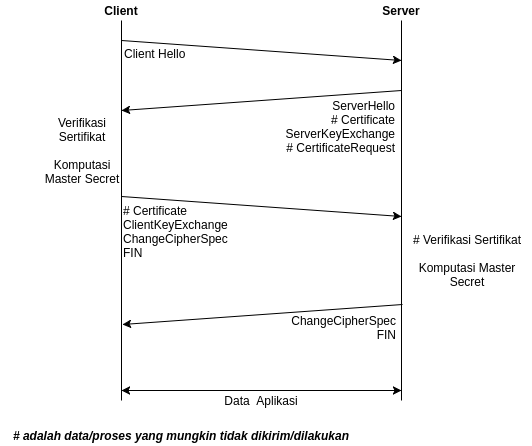
\includegraphics[width=0.6\textwidth]{resources/img/ch-2/handshake.png}
      \caption{Proses Pengiriman Data pada TLS Handshake \protect\citep{rfc5246}}
      \label{fig:tls-handshake}
    \end{figure}

    Pada Gambar ~\ref{fig:tls-handshake}, terlihat bahwa proses handshake merupakan proses yang memakan waktu cukup signifikan. Hal ini disebabkan karena terdapat setidaknya empat kali pengiriman data antara client dan server, selain itu proses \textit{key exchange} dan verifikasi sertifikat yang dilakukan tidak memakan waktu yang singkat.

    Untuk mengatasi hal ini, TLS menyediakan proses handshake singkat dimana client akan menggunakan \textit{session\_id} yang dimilikinya untuk melanjutkan session tersebut. Pada proses ini, client akan mengirimkan data \textit{session\_id} bersama ClientHello; server kemudian akan mencari data session pada session cache dan melanjutkannya jika ditemukan. Jika proses ini gagal, maka proses handshake akan dilakukan seperti biasa. Proses pengiriman data yang dilakukan pada handshake singkat dapat dilihat pada Gambar ~\ref{fig:tls-fast-handshake}.

    \begin{figure}[h]
      \centering
      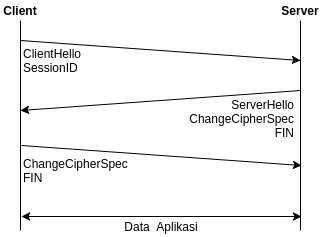
\includegraphics[width=0.6\textwidth]{resources/img/ch-2/fast-handshake.png}
      \caption{Proses Pengiriman Data pada TLS Handshake Singkat \protect\citep{rfc5246}}
      \label{fig:tls-fast-handshake}
    \end{figure}

    Terlihat bahwa penggunaan ulang \textit{session} dapat mempersingkat waktu yang digunakan dalam TLS \textit{handshake} secara signifikan mengingat tidak diperlukannya lagi validasi sertifikat ataupun proses \textit{key exchange}.

  \subsection{Protokol TLS \textit{Record}}
    Protokol TLS \textit{Record} merupakan protokol pemrosesan data yang didapat dari aplikasi untuk kemudian dikirim melalui jaringan dan juga sebaliknya. Ketika TLS menerima data dari sebuah aplikasi, data tersebut akan dibagi menjadi beberapa blok data untuk mempermudah pengolahan, data kemudian akan di-\textit{compress}, ditambahkan MAC, dienkripsi, lalu kemudian dikirim melalui jaringan. Sebaliknya, ketika TLS menerima data dari jaringan, data akan didekripsi, diverifikasi dengan MAC, di-decompress, disusun ulang, lalu dikirim pada aplikasi.

    Pada pengiriman data, TLS menggunakan format data tertentu seperti diilustrasikan pada Gambar ~\ref{fig:tls-record}:
    \begin{figure}[h]
      \centering
      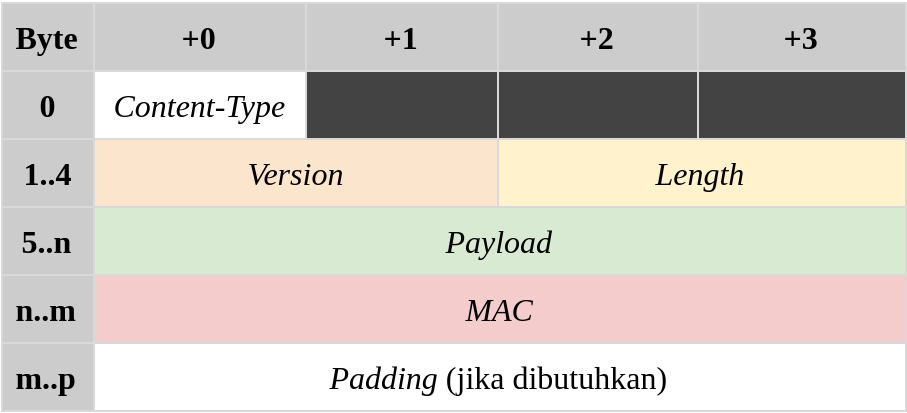
\includegraphics[width=0.6\textwidth]{resources/img/ch-2/tls-record.png}
      \caption{Struktur Sebuah Record TLS \protect\citep{rfc5246}}
      \label{fig:tls-record}
    \end{figure}

    % Untuk setiap koneksi yang ada, TLS akan beberapa nilai yang menggambarkan status dari koneksi tersebut. Salah satu data yang disimpan adalah algoritma kompresi, enkripsi, serta MAC yang digunakan. Selain itu, berbagai parameter yang diperlukan oleh setiap algoritma seperti kunci yang digunakan untuk enkripsi dan MAC juga akan disimpan.

    Proses enkripsi yang terjadi pada tahap ini akan menggunakan sebuah algoritma kriptografi kunci simetris seperti AES ataupun RC4 dengan kunci yang digunakan dalam algoritma tersebut didapatkan oleh client dan server pada TLS Handshake. Penggunaan kriptografi kunci simetris akan membuat proses enkripsi dan dekripsi menjadi relatif lebih cepat jika dibandingkan dengan penggunaan algoritma kriptografi kunci publik.


  \subsection{Ciphersuite}
    \textit{Ciphersuite} adalah sebuah kumpulan dari algoritma yang digunakan dalam TLS \textit{handshake}. Sebuah \textit{ciphersuite} akan terdiri dari algoritma tertentu yang digunakan dalam sebuah koneksi TLS. Kumpulan algoritma tersebut biasanya akan berisi algoritma otentikasi, algoritma \textit{key exchange}, algoritma enkripsi data pada TLS record, serta algoritma MAC. Terdapat banyak kombinasi dari ciphersuite yang umum digunakan pada protokol TLS, beberapa diantaranya memiliki tingkat keamanan yang lebih rendah dibandingkan dengan ciphersuite lain.

    Setiap TLS \textit{client} dan \textit{server} akan memiliki daftar \textit{ciphersuite} yang didukung. Daftar tersebut akan mengurutkan setiap ciphersuite dengan urutan tertentu berdasarkan preferensi dari masing-masing client dan server. Urutan ini biasanya disusun berdasarkan tingkat keamanan dari masing-masing \textit{ciphersuite}. \textit{Ciphersuite} yang memiliki tingkat keamanan tinggi akan memiliki urutan yang lebih prioritas dibandingkan \textit{ciphersuite} dengan tingkat keamanan yang lebih rendah.

    Sebuah ciphersuite biasanya memiliki format penulisan tertentu, sebagai contoh TLS\_DHE\_ RSA\_WITH\_AES\_256\_CBC\_SHA256 adalah \textit{ciphersuite} dengan algoritma key exchange \textit{ephemeral Diffie-Hellman}, algoritma enkripsi simetris AES256, serta SHA256 yang digunakan sebagai algoritma MAC.

    Proses negosisasi ciphersuite antara client dan server dilakukan dengan sederhana. Pertama \textit{ciphersuite} akan dikirim pada pesan ClientHello dan ServerHello. Ketika setiap pihak sudah mendapatkan daftar \textit{ciphersuite} rekannya, ia akan mencari \textit{ciphersuite} tertinggi pada daftar preferensi rekannya dimana ia juga mendukung \textit{ciphersuite} tersebut.
